\documentclass[12pt,letterpaper]{ntdhw}


\usepackage{ntdmath}

\title{Project 1: Regular Languages and Pursuit-Evasion}
\author{CSCI 561}

\rhead{Names:}

%\keytrue

\begin{document}
\pagestyle{fancyplain}

\maketitle
\thispagestyle{fancyplain}
%\clearpage

\begin{figure}
  \centering
  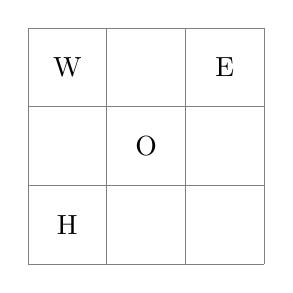
\begin{tikzpicture}
    \draw[step=1cm,gray,very thin,xshift=.5cm,yshift=.5cm] (-1,-1) grid (2,2);
    \node at (0cm,2cm) {W};
    \node at (0cm,0cm) {H};
    \node at (1cm,1cm) {O};
    \node at (2cm,2cm) {E};
  \end{tikzpicture}
  \caption{Example wumpus-world map.  W represents the initial
    location of the wumpus.  H represents the initial location of the
    human.  E represents the escape location.  O represents an
    obstacle that neither the human nor wumpus can move into.}
  \label{fig:map}
\end{figure}

\begin{quote}

\emph{\emph{Pursuit-evasion games} are scenarios with multiple agents
  where one agent attempts to avoid capture by another.  Consider a
  variation of pursuit-evasion games as follows:}

\begin{itemize}
  \item \it Two agents share a grid environment: a human (evader) and wumpus
  (pursuer).
  \item \it The human and wumpus alternate moves on the grid.  The wumpus
  moves each turn up, down, left or right.  The human can move up,
  down, left, right, or remain in place.
  \item \it If the wumpus and human ever occupy the same grid cell,
  the wumpus eats the human.
  \item \it If the human reaches a designed grid cell, they escape.
\end{itemize}

\emph{Answer the following questions using your implementation of finite
automata operations for support.}

\end{quote}

\begin{enumerate}

  \item For the map in \autoref{fig:map}, construct a discrete event
  system model.  Assume that the human's movements are controllable
  and that the wumpus's movements are not controllable.

  \item For your DES model of \autoref{fig:map}, construct a specification
  for the human to avoid the wumpus and escape.
  \begin{enumerate}
    \item Can the human avoid being eaten?  Prove yes or no via
    automata operations.
    \item Can the human escape in finite time (fixed number of steps)?
    Prove yes or no.
  \end{enumerate}

  \item Design a map where the wumpus can always eat the human and
  prove via a DES model that this is the case.

  \item Design a map where the human can always escape and prove via a
  DES model that this is the case.

  \item {\bf Extra Credit:} The previous questions asked you to apply
  regular langauges to the control of discrete event systems.  There
  are many other applications of regular languages (text processing,
  DNA matching, software verification, etc.).  Identify, implement,
  and discuss some other application of regular languages.
\end{enumerate}

\end{document}


%%% Local Variables:
%%% mode: latex
%%% TeX-master: t
%%% End:
